\documentclass[twocolumn]{article}
\usepackage[utf8]{inputenc}

\usepackage{algcompatible}
\usepackage{algorithm}
\usepackage{algpseudocode}
\usepackage{amsmath}
\usepackage{graphicx}
\usepackage{hyperref}
\usepackage{subcaption}

\graphicspath{ {./figures/} }

\title{High-Dimensional Data Stream Visualization}
\author{Chanon Jenakom}
\date{8 April, 2019}

\begin{document}

\maketitle

\section{Introduction}

In recent times, there are many sources of data that can be used for performing data analysis on.
Most of these data contain so many features and attributes that contribute to the meaning of
each piece of data, such as churn detection in microblogs \cite{churn_microblog} and financial
analysis \cite{multidimensional_visualization_1}. Moreover, sources of these kinds of data are
usually from social media sites such as Twitter, which is also provided as streams. Streaming data
introduces more constraining characteristics to the problem: dynamic, continuous and unbounded
\cite{stream_mining_survey}.

Many high-dimensional data visualization methods have been proposed over the years to
extract meaningful patterns from the data \cite{multidimensional_visualization_1}. One of the
earliest methods used were various types of graphs \cite{multidimensional_visualization_2}. For an
example, a matrix of scatter plots can be used to visualize the pairs of attributes within the
data. Another technique used is a popular dimensionality reduction technique called Principal
Component Analysis (PCA) \cite{pca}. While effective in creating a subset of independent features
that represent the original data, this method is not capable of consistently capturing both the
local and global structures of the data \cite{tsne}. However, another technique called
t-Distributed Stochastic Neighbor Embedding, or t-SNE, is capable of capturing various structures
of the high-dimensional data considerably well.

Despite of the fact that there are many visualizing algorithms proposed in the field, only a
selected few are specifically designed to visualize streaming data. Most are modified versions of
pre-existing techniques adapted for streaming environments, such as a suggestion provided in
\cite{atsne} or GPU-accelerated version of t-SNE \cite{tsne_cuda}, or a new PCA implementation,
named History PCA \cite{hist_pca}.

In this paper, each high-dimensional data visualization techniques are reviewed and compared in
details. Each section will explore the performance of each technique on MNIST Digits dataset, and
its possibility in being used in streaming contexted is discussed.

\section{Algorithms}

In this section, the brief history of data visualization in high dimension is discussed. Moreover,
each of the techniques that is effective and popular is reviewed in terms of its mathematical and
statistical foundation and its visualization quality, using the digits dataset as shown in Figure
\ref{fig:digits}.

\begin{figure}[hbt]
  \centering
  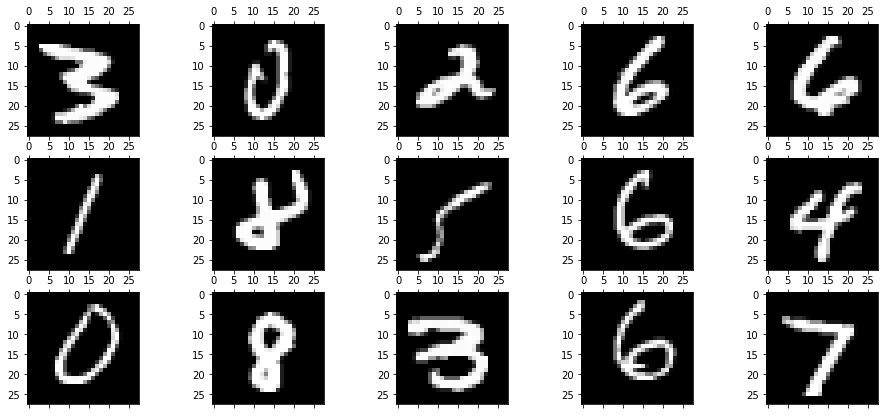
\includegraphics[width=6.5cm, height=3.9cm]{digits.png}
  \caption{Examples of MNIST Digits}
  \label{fig:digits}
\end{figure}

\subsection{History}

In order to perform visualization on high-dimensional data, there have been many techniques and
algorithms proposed. Ranging from simple graphs such as scatter plots or heatmaps
\cite{multidimensional_visualization_2} to more complex methods that rely on statistical theories
such as PCA \cite{pca} and t-SNE \cite {tsne}. These varying techniques offer different use cases
and strengths and weaknesses when presented with different sets of data.

\subsection{Principal Component Analysis}

Principal Component Analysis is a statistical procedure that convert a set of observations of
possibly correlated variables into a set of values of linearly uncorrelated variables called
principal components \cite{pca}. While used mostly as a tool for making predictive models, it has
also been used to visualize genetic distance and relatedness between data points.

PCA can be thought of as fitting a p-dimensional ellipsoid to the data, where each of the axis of
the ellipsoid represents a principal component, as show in Figure \ref{fig:pca_technical}. The size
of the axis corresponds to the variance along that axis, which signifies to contribution the
component has to the overall meaning of the dataset.

\begin{figure}[hbt]
  \centering
  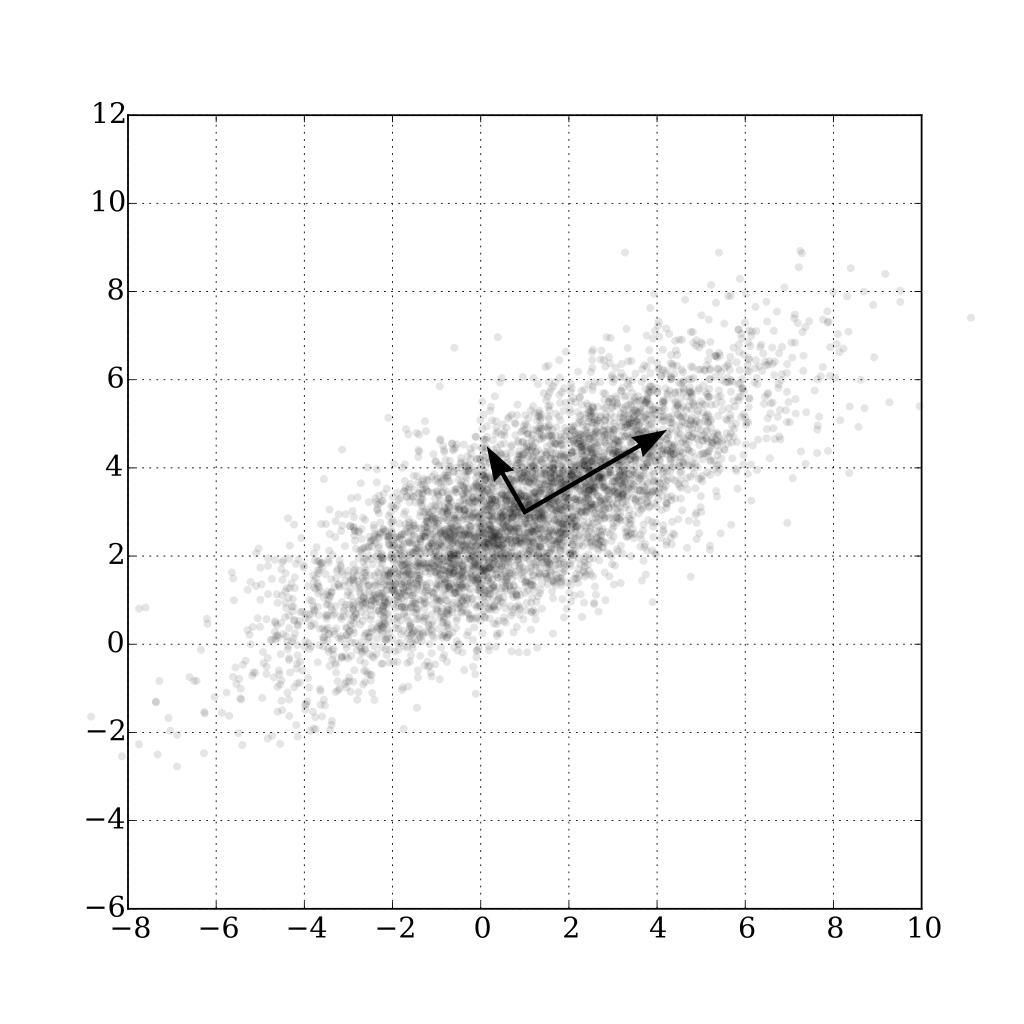
\includegraphics[width=7cm, height=5.4cm]{pca_technical.png}
  \caption{Principal Component Analysis on 2D Data}
  \label{fig:pca_technical}
\end{figure}

The first principal component is very important to this algorithm, whose variance must be maximized.
Thus, the first weight vector has tp satisfy the following formula:

\begin{equation}
  w_{(1)} = \operatorname*{argmax}{\frac{w^TX^TXw}{w^Tw}}
  \label{eqn:first_component}
\end{equation}

and every further $k^{th}$-component has to satisfy the following formula:

\begin{equation}
  \hat{X}_k = X - \sum_{s=1}^{k-1} Xw_{(s)}w^T_{(s)}
  \label{eqn:kth_component}
\end{equation}

When used on MNIST digits dataset, as seen in Figure \ref{fig:pca}, it can be seen that the separation
between digits are not apparent as expected. There is no distinct separation between digits, and
most are even placed on the same space within the xy-plane.

\begin{figure}[hbt]
  \centering
  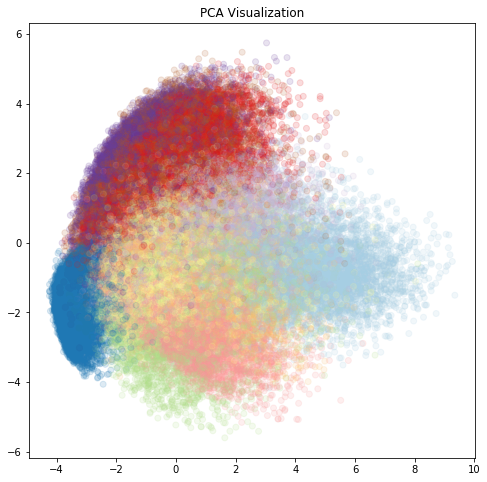
\includegraphics[width=7cm, height=5.4cm]{pca.png}
  \caption{PCA on MNIST Digits Dataset}
  \label{fig:pca}
\end{figure}

\subsection{t-Distrubuted Stochastic Neighbor Embedding}

t-Distributed Stochastic Neighbor Embedding, or t-SNE, uses the concept of probability to reduce the
dimensions of high-dimensional data and is able to construct a reasonably good visualizations
\cite{tsne}. The main idea of t-SNE is to map distances in high-dimensional space to
probabilities, then minimize the mappings of these probabilities in low-dimensional space,
following the cost function:

\begin{equation}
  C = KLP(P||Q) = \sum_i\sum_jp_{ij}\log\frac{p_{ij}}{q_{ij}}
  \label{eqn:klp}
\end{equation}

which is the sum of Kullback-Leibler divergences \cite{klp}. The algorithm is shown here:

\begin{algorithm*}
  \textbf{Data}: data set $X = \{x_1,x_2,...,x_n\}$, \\
  \textbf{Result}: low-dimensional data representation $\gamma^{(T)} = \{y_1,y_2,...,y_n\}$ \\
  \textbf{begin}
  \begin{algorithmic}[1]
    \State $p_{ij} \gets \frac{p_{j|i}+p_{i|j}}{2n}$
    \State $\gamma^{(0)} \gets \{y_1,y_2,...,y_n\}$
    \For{$t \gets 1$ to $T$}
      \State $q_{ij} \gets \frac{{(1+{||y_i-y_j||}^2)}^{-1}}{\sum_{k \neq 1} {(1+{||y_k-y_l||}^2)}^{-1}}$
      \State $\frac{\delta C}{\delta \gamma_i} \gets 4 \sum_j (p_{ij}-q{ij})(y_i-y_j){(1+{||y_i-y_j||}^2)}^{-1}$
      \State $\gamma^{(t)} \gets \gamma^{t-1} + \eta \frac{\delta C}{\delta \gamma_i}+\alpha(t)(\gamma^{(t-1)}-\gamma^{(t-2)})$
    \EndFor
  \end{algorithmic}
  \caption{Simple version of t-Distributed Stochastic Neighbor Embedding}
\end{algorithm*}

\pagebreak

When used on MNIST digits dataset, as seen in Figure \ref{fig:tsne}, clear distinctions are shown
between digits. However, the digits are still close together and indistinguishable in some areas of
the 2-dimensional plane. Thus, PCA, or any other dimensionality reduction technique, can be used to
extract more relevant features from the data before being fed into t-SNE algorithm.

\begin{figure}[t!]
  \centering
  \begin{subfigure}[t]{0.5\textwidth}
    \centering
    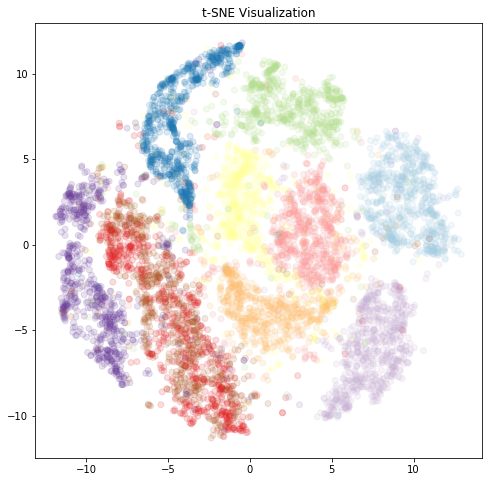
\includegraphics[width=6cm, height=4.9cm]{tsne.png}
    \caption{Without PCA}
  \end{subfigure}
  \begin{subfigure}[t]{0.5\textwidth}
    \centering
    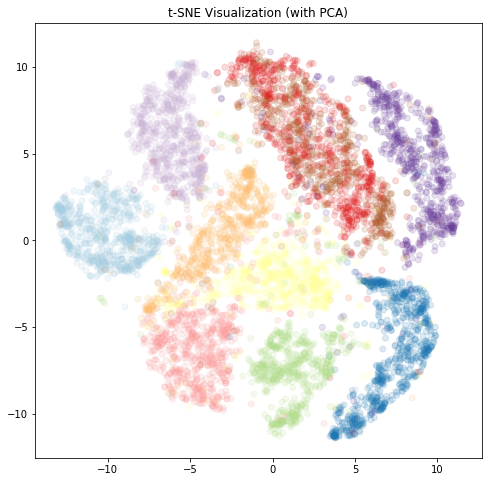
\includegraphics[width=6cm, height=4.9cm]{tsne_with_pca.png}
    \caption{With PCA}
  \end{subfigure}
  \caption{t-SNE on MNIST Digits Dataset}
  \label{fig:tsne}
\end{figure}

\section{Conclusion}

\begin{table}[hbt]
  \caption{Data Visualization Comparison}
  \begin{center}
    \begin{tabular}{l r r}
      \hline
      \textbf{Algorithm} & \textbf{Digits Separation} & \textbf{Incremental?} \\
      \hline
      PCA & Poor & Yes \\
      t-SNE & Good & No \\
      t-SNE \& PCA & Excellent & No \\
      \hline
    \end{tabular}
    \label{tbl:comparison}
  \end{center}
\end{table}

According to the resultant visualizations, it can be concluded to between Principal Component
Analysis and t-Distributed Stochastic Neighbor Embedding, the latter performs remarkably well in
mapping high-dimensional data into low-dimensional data for ease of visualization. Moreover, both
methods can be used together to further improve the quality of the data visualization.

Upon further studies regarding the abilities and limitations of each of these data visualization
algorithms, it was found that PCA and its variants are able to perform data visualization using
previously fed data, which means that the previous results are combined with new ones to create a
continuous visualization of data. However, this is not true in the original implementation of t-SNE.

\begin{figure}[t!]
  \centering
  \begin{subfigure}[t]{0.5\textwidth}
    \centering
    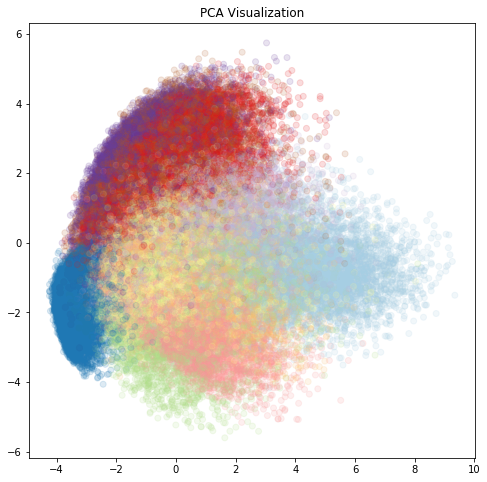
\includegraphics[width=6cm, height=4.9cm]{pca.png}
    \caption{PCA}
  \end{subfigure}
  \begin{subfigure}[t]{0.5\textwidth}
    \centering
    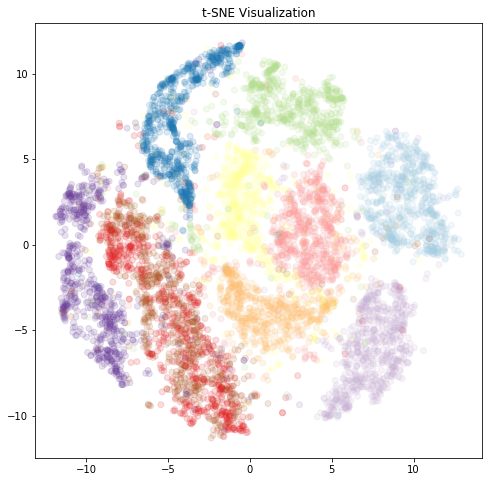
\includegraphics[width=6cm, height=4.9cm]{tsne.png}
    \caption{t-SNE}
  \end{subfigure}
  \begin{subfigure}[t]{0.5\textwidth}
    \centering
    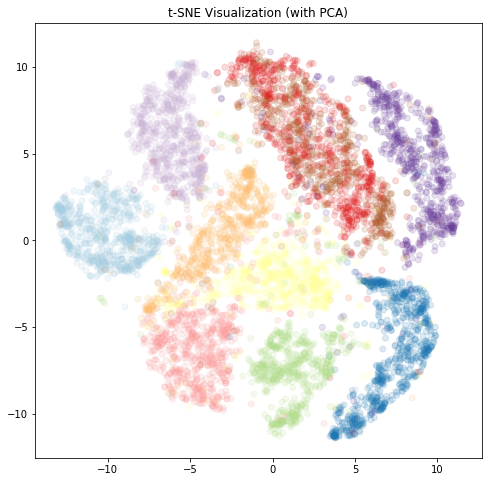
\includegraphics[width=6cm, height=4.9cm]{tsne_with_pca.png}
    \caption{t-SNE \& PCA}
  \end{subfigure}
  \caption{MNIST Digits Dataset Visualizations}
  \label{fig:comparison}
\end{figure}

\bibliographystyle{unsrt}
\bibliography{refs}

\end{document}
